\documentclass{article}

% Language setting
% Replace `english' with e.g. `spanish' to change the document language
\usepackage[spanish]{babel}

% Set page size and margins
% Replace `letterpaper' with `a4paper' for UK/EU standard size
\usepackage[letterpaper,top=2cm,bottom=2cm,left=3cm,right=3cm,marginparwidth=1.75cm]{geometry}

% Useful packages
\usepackage{amsmath}
\usepackage{graphicx}
\usepackage{enumitem}
\usepackage{comment}
\usepackage{wrapfig}
\usepackage[colorlinks=true, allcolors=blue]{hyperref}

\title{Redes Tema 2. Capa de aplicación}
\author{Martín González Dios 
\href{https://github.com/martindios}{\includegraphics[height=0.5cm]{github.png}}}

\begin{document}
\maketitle

Se ocupa de la \textbf{comunicación entre procesos}, para lo que usa protocolos de comunicación que permiten la comprensión de los mensajes y facilitan la programación de funciones de envío y recepción. Deben especificar el \textbf{tipo de mensaje} (petición, respuesta, ...), \textbf{reglas sobre el cuándo y cómo se envían los mensajes}, la \textbf{sintaxis del mensaje} (campos) y la semántica de cada campo. Usan \textbf{protocolos básicos de la capa de transporte y necesitan saber si usan TCP o UDP}, el ancho de banda y la temporización.

\textbf{Agente de usuario}: Interfaz entre usuario y aplicación (navegador, gestor de correo, ...).

\begin{figure}[h]
    \centering
    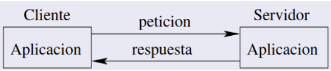
\includegraphics[width=0.4\textwidth]{img-t1/img_576_57.png}
\end{figure}

\section{HTTP}

El 	\textbf{Protocolo de Transferencia de Hipertexto (HTTP)} define la comunicación entre un servidor web y un cliente web. Este protocolo utiliza el protocolo \textbf{TCP} y opera sobre el puerto \textbf{80}. Aunque HTTP es intrínsecamente \textit{sin estado}, el uso de cookies permite dar la sensación de persistencia.

\subsection{Estructura de una página web}

Una página web consiste en un \textbf{documento HTML base}, que define la distribución y el texto, junto con varios \textbf{objetos} adicionales (archivos direccionables mediante URLs). 

\begin{itemize}
    \item El \textbf{navegador} actúa como el agente de usuario para la web.
    \item El \textbf{servidor web} alberga los objetos y responde a las solicitudes del cliente.
    \item Ante una solicitud de una página web, el servidor devuelve el documento base acompañado de sus objetos asociados.
\end{itemize}

\subsection{Conexiones HTTP}

Las conexiones HTTP pueden clasificarse en dos tipos:

\begin{itemize}
    \item \textbf{Conexiones no persistentes:} Se utiliza una conexión TCP diferente para transferir cada objeto. Esto puede hacerse:
    \begin{itemize}
        \item En serie: Cada objeto se transfiere esperando a que la conexión previa se cierre.
        \item En paralelo: Varias conexiones se abren simultáneamente para transferir objetos.
    \end{itemize}

    \item \textbf{Conexiones persistentes:} Se utiliza una única conexión TCP para transferir múltiples objetos e incluso páginas completas. Dentro de este tipo, encontramos:
    \begin{itemize}
        \item \textbf{Sin entubamiento (sin pipelining):} El cliente solicita un nuevo objeto solo después de recibir el anterior.
        \item \textbf{Con entubamiento (con pipelining):} El cliente puede realizar múltiples solicitudes de objetos sin esperar a recibir los anteriores.
    \end{itemize}
\end{itemize}

\subsection{Tiempo de transferencia de una página web}

El tiempo de transferencia de una página web depende de:

\begin{itemize}
    \item El \textbf{RTT} (Round-Trip Time), que es el tiempo de ida y vuelta cliente-servidor-cliente.
    \item El tiempo de \textbf{transmisión del archivo}, que depende del tamaño del archivo.
\end{itemize}

Para el primer paquete, el tiempo total es de $2 \times RTT + t_{\text{transmisión}}$. Para los paquetes restantes, el tiempo depende del tipo de conexión utilizada.

\newpage

\subsection{Mensajes HTTP}

Los mensajes HTTP están compuestos por:

\begin{itemize}
    \item \textbf{Cabecera:} Contiene información de control en formato ASCII (7 bits).
    \item \textbf{Cuerpo:} Contiene los datos, que pueden estar en formato binario.
\end{itemize}

Existen dos tipos de mensajes:

\subsubsection{Mensajes de petición}

\begin{itemize}
    \item \textbf{Línea de petición:} Especifica el objeto solicitado. Ejemplos:
    \begin{itemize}
        \item \texttt{GET}: Solicitud de una página normal.
        \item \texttt{POST}: Envío de datos desde un formulario.
    \end{itemize}

    \item \textbf{Líneas de cabecera (opcionales):} Ejemplos de campos incluyen:
    \begin{itemize}
        \item \texttt{Host}
        \item \texttt{Connection}
        \item \texttt{User-Agent}
        \item \texttt{Language}
    \end{itemize}

    \item \textbf{Cuerpo:} Vacío para \texttt{GET} y con datos del formulario para \texttt{POST}.
\end{itemize}

\subsubsection{Mensajes de respuesta}

\begin{itemize}
    \item \textbf{Línea de estado:} Indica el estado de la respuesta. Ejemplos de códigos:
    \begin{itemize}
        \item \texttt{200}: Éxito.
        \item \texttt{404}: No encontrado.
        \item \texttt{400}: Solicitud incorrecta.
    \end{itemize}

    \item \textbf{Líneas de cabecera (opcionales):} Ejemplos de campos incluyen:
    \begin{itemize}
        \item \texttt{Connection}
        \item \texttt{Date}
        \item \texttt{Server}
        \item \texttt{Last-Modified}
        \item \texttt{Content-Length}
        \item \texttt{Content-Type}
    \end{itemize}

    \item \textbf{Cuerpo:} Contiene los datos de la respuesta.
\end{itemize}

\subsection{HTTP/2}

Con la llegada de HTTP/2 se introdujeron muchas mejoras respecto a la versión anterior:

\begin{itemize}
    \item Multiplexación de múltiples peticiones HTTP sobre una misma conexión TCP.
    \item Compresión de cabeceras para reducir el tamaño de las transmisiones.
    \item Soporte para \textbf{server push}, que permite al servidor enviar recursos adicionales sin solicitud explícita del cliente.
    \item Pipelining de solicitud-respuesta.
    \item Cifrado obligatorio mediante SSL (Secure Sockets Layer).
    \item Incremento de velocidad: HTTP/2 es un 65\% más rápido que HTTP/1.1.
\end{itemize}

\newpage

\section{FTP}

El 	\textbf{Protocolo de Transferencia de Archivos (FTP)} es un protocolo que define la comunicación entre un cliente y un servidor de archivos. Este protocolo es 	\textbf{con estado}, manteniendo la sesión activa durante toda la comunicación, y utiliza dos conexiones TCP paralelas para su funcionamiento. 

\subsection{Conexiones FTP}

FTP emplea dos tipos de conexiones TCP:

\begin{itemize}
    \item \textbf{Conexión de control:} 
    \begin{itemize}
        \item Utiliza el puerto \textbf{21}.
        \item Es \textbf{persistente}, permaneciendo activa durante toda la sesión.
        \item Se emplea para enviar comandos y recibir respuestas. Los comandos son cadenas de 4 caracteres en mayúscula, acompañadas de campos adicionales. Algunos ejemplos de comandos son:
        \begin{itemize}
            \item \texttt{USER}: Especifica el nombre de usuario.
            \item \texttt{PASS}: Especifica la contraseña.
            \item \texttt{RETR}: Solicita la descarga de un archivo.
        \end{itemize}
        \item Las respuestas consisten en códigos de 3 dígitos seguidos de una frase explicativa. Algunos ejemplos de códigos de respuesta son:
        \begin{itemize}
            \item \texttt{331}: Se requiere una contraseña.
            \item \texttt{125}: La transferencia de datos está en progreso.
            \item \texttt{425}: No se pudo abrir la conexión de datos.
        \end{itemize}
        \item Utiliza el formato ASCII de 7 bits para la comunicación.
    \end{itemize}

    \item \textbf{Conexión de datos:}
    \begin{itemize}
        \item Utiliza el puerto \textbf{20}.
        \item Es \textbf{no persistente}, abriéndose una nueva conexión para cada archivo que se transmite.
        \item Se emplea para transferir los datos en respuesta a los comandos recibidos a través de la conexión de control.
        \item También utiliza el formato ASCII de 7 bits para la transferencia de datos.
    \end{itemize}
\end{itemize}

\subsection{Seguridad en FTP}

Es importante destacar que FTP, al igual que Telnet y HTTP, no cifran las comunicaciones, lo que los hace vulnerables a intercepciones. Por el contrario, protocolos como SFTP, SSH y HTTPS cifran las conexiones, garantizando una mayor seguridad durante la transferencia de información.

\newpage

\section{Protocolos de correo electrónico}

En el ámbito del correo electrónico, se utilizan diferentes protocolos para el envío y acceso a los mensajes. Los principales protocolos son \textbf{SMTP}, \textbf{POP3}, \textbf{IMAP}, y HTTP (cuando se utiliza un navegador para acceder al correo). Estos protocolos operan de la siguiente manera:

\subsection{SMTP (Protocolo simple de transferencia de correo)}
SMTP es el protocolo utilizado para enviar correo electrónico al servidor de correo o entre servidores. Este protocolo permite la comunicación entre el agente de usuario y el servidor de correo. Si el servidor de destino no está disponible, se realiza un reintento después de un intervalo de 30 minutos.

\begin{itemize}
    \item \textbf{Puerto}: 25.
    \item \textbf{Conexión}: TCP persistente, es decir, se mantienen abiertas para varios mensajes.
    \item \textbf{Codificación}: Se utiliza ASCII de 7 bits para las cabeceras y los cuerpos de los mensajes.
    \item \textbf{Mensajes}: Existen tres tipos de mensajes en SMTP:
    \begin{itemize}
        \item \textbf{Comandos}: Palabras en mayúsculas seguidas de parámetros, como \texttt{HELO}, \texttt{MAIL FROM}, entre otros.
        \item \textbf{Respuestas}: Códigos numéricos seguidos de una frase, como \texttt{220}, \texttt{354}, \texttt{221}, etc.
        \item \textbf{Datos}: El contenido de los correos electrónicos.
    \end{itemize}
    \item \textbf{Seguridad}: SMTP es un protocolo inseguro ya que no requiere autenticación (no pide nombre de usuario ni contraseña), lo que facilita el envío de correos electrónicos no solicitados.
    \item \textbf{Naturaleza}: SMTP es un protocolo de oferta, en el que el cliente ofrece el mensaje al servidor, a diferencia de HTTP, que es de demanda. Además, SMTP requiere que los correos sean codificados en ASCII de 7 bits (a diferencia de HTTP que permite datos binarios).
    \item \textbf{Estado}: SMTP mantiene el estado de la sesión, lo que significa que recuerda la fase en la que se encuentra durante la transferencia de correos.
\end{itemize}

\subsection{POP3 (Protocolo de oficina postal versión 3)}
POP3 es un protocolo más sencillo que SMTP, utilizado para acceder a los correos electrónicos mediante una conexión TCP persistente. Opera sin mantener estado entre las sesiones.

\begin{itemize}
    \item \textbf{Puerto}: 110.
    \item \textbf{Fases del protocolo}:
    \begin{itemize}
        \item \textbf{Autorización}: En esta fase, se autentica al usuario con su nombre de usuario y contraseña.
        \item \textbf{Transacción}: Se recuperan los mensajes del servidor, se marcan los correos para su borrado y se recopilan estadísticas sobre el correo.
        \item \textbf{Actualización}: Se eliminan los mensajes marcados para borrar y se finaliza la sesión.
    \end{itemize}
    \item \textbf{Comandos}: Los comandos en POP3 son palabras de 4 caracteres seguidas de parámetros, como \texttt{USER}, \texttt{PASS}, \texttt{LIST}, entre otros.
    \item \textbf{Respuestas}: Las respuestas del servidor son \texttt{+OK} (si la operación fue exitosa) o \texttt{-ERR} (si ocurrió un error).
    \item \textbf{Datos}: Los datos incluyen la lista de mensajes y el contenido de los correos. A diferencia de SMTP, POP3 entrega el correo completo en un solo mensaje, no de forma fragmentada.
\end{itemize}

\subsection{IMAP (Protocolo de acceso a mensajes de Internet)}
IMAP es un protocolo más avanzado que POP3. A diferencia de POP3, IMAP permite una mayor flexibilidad en el acceso y gestión de los correos electrónicos.

\begin{itemize}
    \item \textbf{Carpetas}: IMAP asocia cada mensaje con una carpeta, lo que permite una organización más eficiente de los correos. POP3 no ofrece soporte para carpetas.
    \item \textbf{Comandos avanzados}: IMAP incluye comandos para crear carpetas, realizar búsquedas en los correos electrónicos, y más.
    \item \textbf{Estado entre sesiones}: IMAP mantiene el estado entre sesiones, lo que significa que conserva la información sobre la posición y el estado de los mensajes entre sesiones, algo que POP3 no permite.
    \item \textbf{Conexión}: Como POP3, IMAP utiliza una conexión TCP persistente, pero permite un acceso más completo y organizado al correo.
\end{itemize}

\section{DNS (Servicio de Nombres de Dominio)}

El DNS (Domain Name System) es un sistema que \textbf{traduce los nombres de host a direcciones IP y viceversa}. Además, tiene varias funciones importantes, como obtener alias, informar sobre los servidores autorizados para un dominio, proporcionar alias de servidores de correo y distribuir la carga mediante la asignación de varias direcciones IP a un nombre de host.

\begin{itemize}
    \item \textbf{Funciones principales del DNS}:
    \begin{itemize}
        \item Traduce nombres de hosts a direcciones IP.
        \item Obtiene alias y proporciona alias de servidores de correo, lo que simplifica las direcciones.
        \item Informa sobre los servidores autorizados para un dominio.
        \item Distribuye la carga asignando varias direcciones IP a un solo nombre de host, utilizando servidores espejo y devolviendo cíclicamente una de las IPs asignadas.
    \end{itemize}
    \item \textbf{Estructura del DNS}:
    \begin{itemize}
        \item El sistema DNS está compuesto por servidores de nombres distribuidos a través de Internet.
        \item Utiliza una base de datos jerárquica para almacenar la información.
        \item Opera bajo un protocolo UDP sin estado, utilizando el puerto 53.
    \end{itemize}
    \item \textbf{Tipos de servidores DNS}:
    \begin{itemize}
        \item \textbf{Servidores locales}: Atienden las consultas realizadas por los hosts en la red local.
        \item \textbf{Servidores autorizados o autoritativos}: Registran los hosts en dos servidores autorizados para que sean accesibles en Internet. Estos servidores pertenecen al ISP (Proveedor de Servicios de Internet) y muchos actúan como servidores locales.
        \item \textbf{Servidores raíz}: Más de 400 servidores gestionados por 13 organizaciones. Tienen la información sobre los dominios de primer nivel (TLD).
        \item \textbf{Servidores intermedios o TLD}: Contienen información sobre los niveles intermedios en la jerarquía de dominios.
    \end{itemize}
    \item \textbf{Caché de DNS}:
    \begin{itemize}
        \item En todos los niveles, los servidores DNS almacenan copias de las correspondencias que obtienen. Estos datos se borran después de cierto tiempo si no se utilizan.
    \end{itemize}
\end{itemize}

\subsection{Mensajes DNS}

Los mensajes DNS se componen de una consulta y una respuesta, y están organizados de la siguiente manera:

\begin{itemize}
    \item \textbf{Cabecera}: Contiene la información de control, incluyendo:
    \begin{itemize}
        \item \textbf{Identificación}: 16 bits que identifican la consulta.
        \item \textbf{Señales}: 4 bits que indican si se trata de una consulta o una respuesta y el tamaño de los campos.
    \end{itemize}
    \item \textbf{Cuerpo}: Contiene las siguientes secciones:
    \begin{itemize}
        \item \textbf{Cuestiones}: Información solicitada por la consulta.
        \item \textbf{Respuestas}: Respuestas a la consulta.
        \item \textbf{Servidores autorizados}: Información sobre los servidores DNS autorizados.
        \item \textbf{Información adicional}: Datos adicionales que pueden ser útiles.
    \end{itemize}
\end{itemize}

\subsection{Tipos de consultas DNS}

Las consultas DNS pueden ser de dos tipos:

\begin{itemize}
    \item \textbf{Consultas recursivas}: En este tipo de consultas, cada servidor DNS pregunta al siguiente hasta obtener una respuesta final.
    \item \textbf{Consultas reiterativas}: En este caso, el servidor DNS local contacta con todos los servidores DNS involucrados, obteniendo respuestas directas de cada uno.
\end{itemize}

\begin{figure}[h]
    \centering
    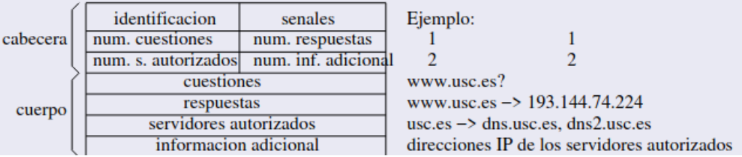
\includegraphics[width=0.75\textwidth]{img-t1/img_285_32.png}
\end{figure}

\section{Distribución de Contenidos}

El acceso a servidores centralizados puede ser lento debido a factores como caminos lentos, congestión de la red o servidores sobrecargados. Para mitigar esto, se distribuyen y duplican los contenidos en varias zonas, y las peticiones se dirigen al servidor que ofrezca el menor tiempo de respuesta.

\subsection{Caché Web o Servidor Proxy}

Un método común de distribución es la \textbf{caché web}, también conocida como \textbf{servidor proxy}. Este método es proporcionado por el ISP (Proveedor de Servicios de Internet) y se basa en un servidor intermedio (proxy) por el cual pasan las peticiones web de los hosts dentro de una red. El servidor proxy mantiene copias de los contenidos temporalmente, lo que mejora el tiempo de acceso a los recursos solicitados. Además, permite establecer un esquema jerárquico. Sin embargo, el usuario debe configurar su navegador para utilizar este método.

\subsection{Redes de Distribución de Contenidos (CDN)}

Otro enfoque de distribución es el uso de \textbf{Redes de Distribución de Contenidos} (\textbf{CDN}, por sus siglas en inglés). Este sistema se basa en empresas que poseen centros de hosting de Internet (compañías CDN) y alquilan su infraestructura. La CDN replica los contenidos de sus clientes en sus propios servidores y se asegura de que estos estén actualizados. 

El contenido se entrega desde el \textbf{servidor CDN} que pueda ofrecer el acceso más rápido, lo cual mejora el rendimiento y la disponibilidad. El acceso a los contenidos puede ser realizado a través de \textbf{redirección de objetos} o mediante \textbf{balanceo de las peticiones}, utilizando el sistema DNS para dirigir las solicitudes al servidor más cercano o rápido.

\subsection{Redes P2P (Peer-to-Peer)}

Las \textbf{redes P2P} permiten que todos los usuarios actúen tanto como servidores como clientes mediante el uso de una aplicación. Este modelo elimina la necesidad de servidores centralizados, ya que los usuarios comparten directamente los contenidos entre sí.

Para su funcionamiento, una red P2P necesita un \textbf{nodo de arranque} y un \textbf{directorio} que puede ser centralizado, no centralizado o basado en la inundación de consultas.

\subsubsection{BitTorrent}

Con el protocolo \textbf{BitTorrent}, cada archivo se comparte dentro de una red P2P específica que no requiere un directorio centralizado. En lugar de ello, la información de los archivos se almacena en archivos \textbf{.torrent}, que contienen los detalles necesarios para que los usuarios puedan localizar y compartir los contenidos. Aunque no es necesario un directorio, el sistema BitTorrent sí necesita un \textbf{tracker} para cada red, el cual ayuda a coordinar las descargas y mantener la conexión entre los usuarios que comparten los archivos.




\begin{comment}
\begin{figure}[h]
    \centering
    \includegraphics[width=0.5\textwidth]{1.png}
    \caption{}
\end{figure}
\end{comment}

\begin{comment}
\begin{wrapfigure}[]{r}{0.5\linewidth}
    \centering
    \includegraphics[width=\linewidth]{8.png}
    \caption{}
\end{wrapfigure}
\end{comment}

\end{document}